The prototype which Aveiro people designed is quite similar to the prototype which was designed by Valencia people but it has a few difference which is very important from point of view of physics. 

Both prototypes are formed for a external cilinder whose material is teflon. The impotance to use teflon here is that the fibers which we use in our experiment (BCF-12) have a emision spectrum with a peak at $\lambda=435~\nm$ and the reflection coefficient which have the teflon is close to 1 for this type of photons. 

In the Figure \ref{externalcilinder} I show you this external cilinder whose length is $200~\mm$. It's internal and external diameter is $43~\mm$ and $61~\mm$ respectively. Moreover this cilinder have two holes like the hole which appear in the figure \ref{hole}. We will use this holes for filling and emptying this prototype which tritium water. You have to take into account that you need two holes every time that you fill or empty your prototype because you will use one out of this holes for filling or emptying your prototype and the other hole for emptying or filling the air your prototype respectively.

\begin{figure}[hbtp]
 \centering
  \subfloat[]{
    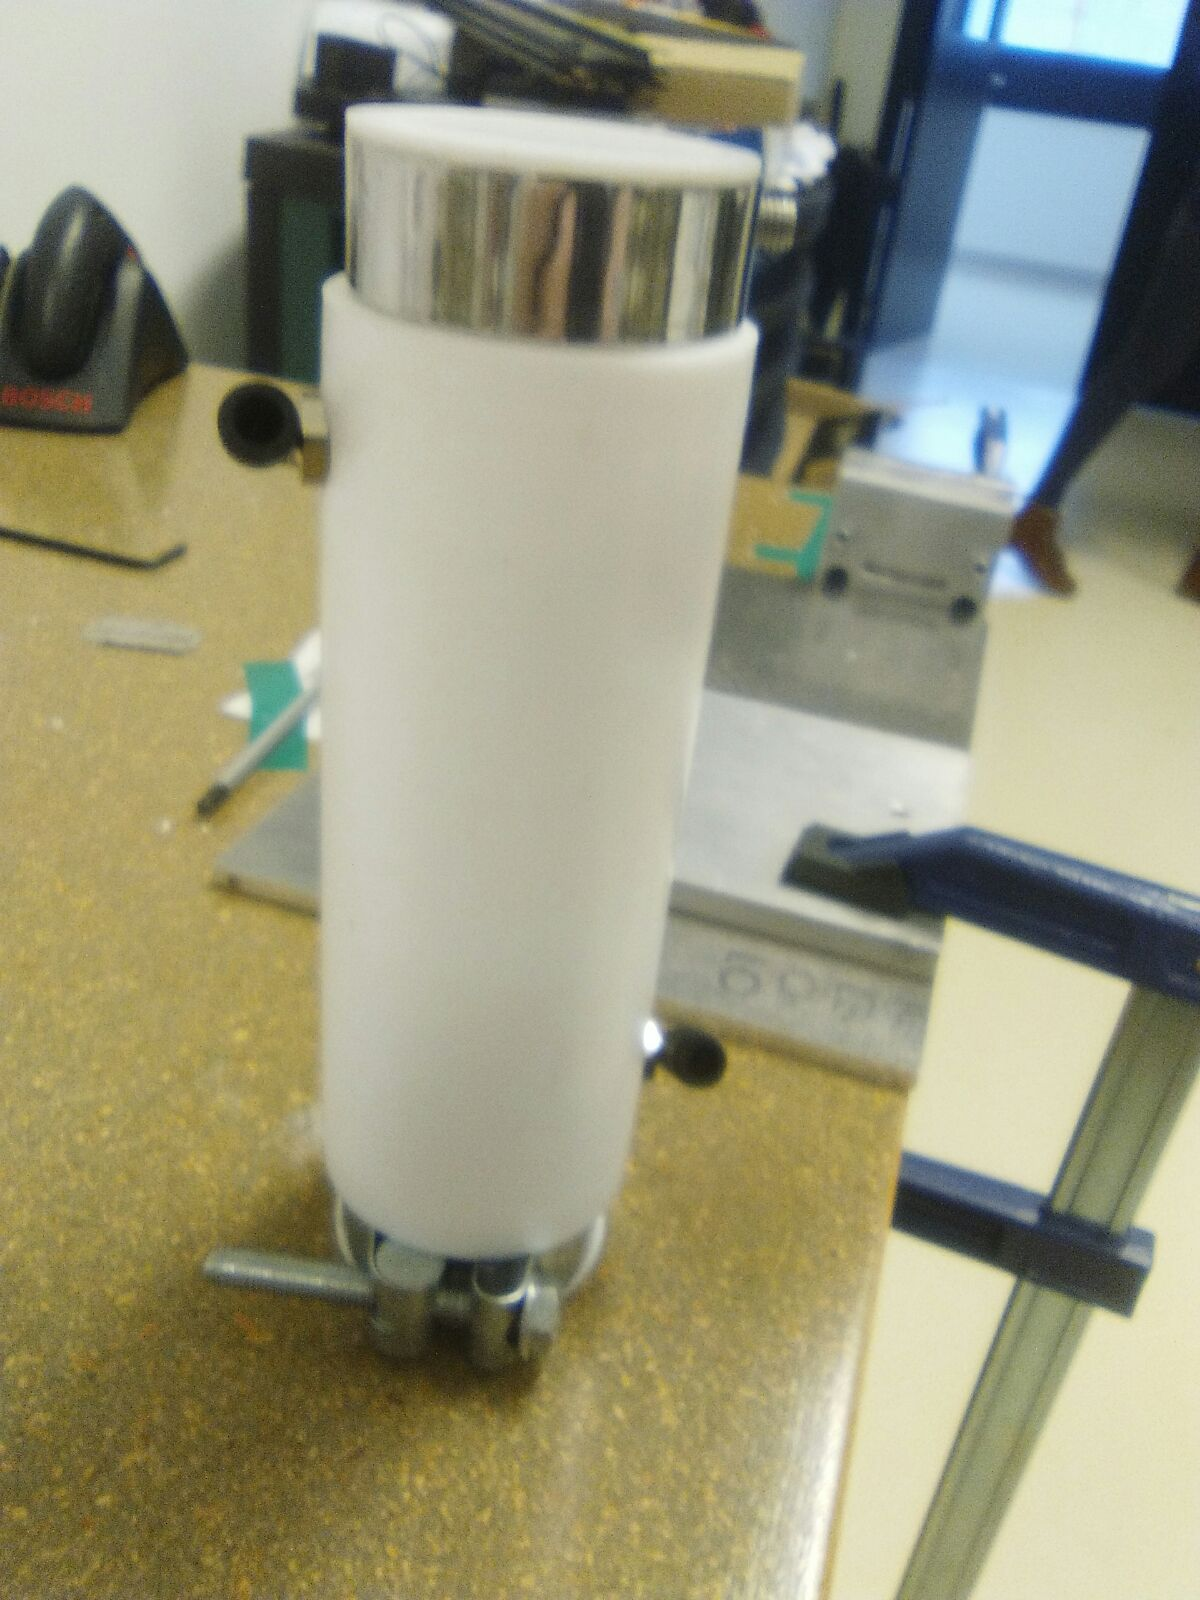
\includegraphics[width=0.5 \textwidth]{AveiroPrototype.jpeg}}
  \subfloat[]{
    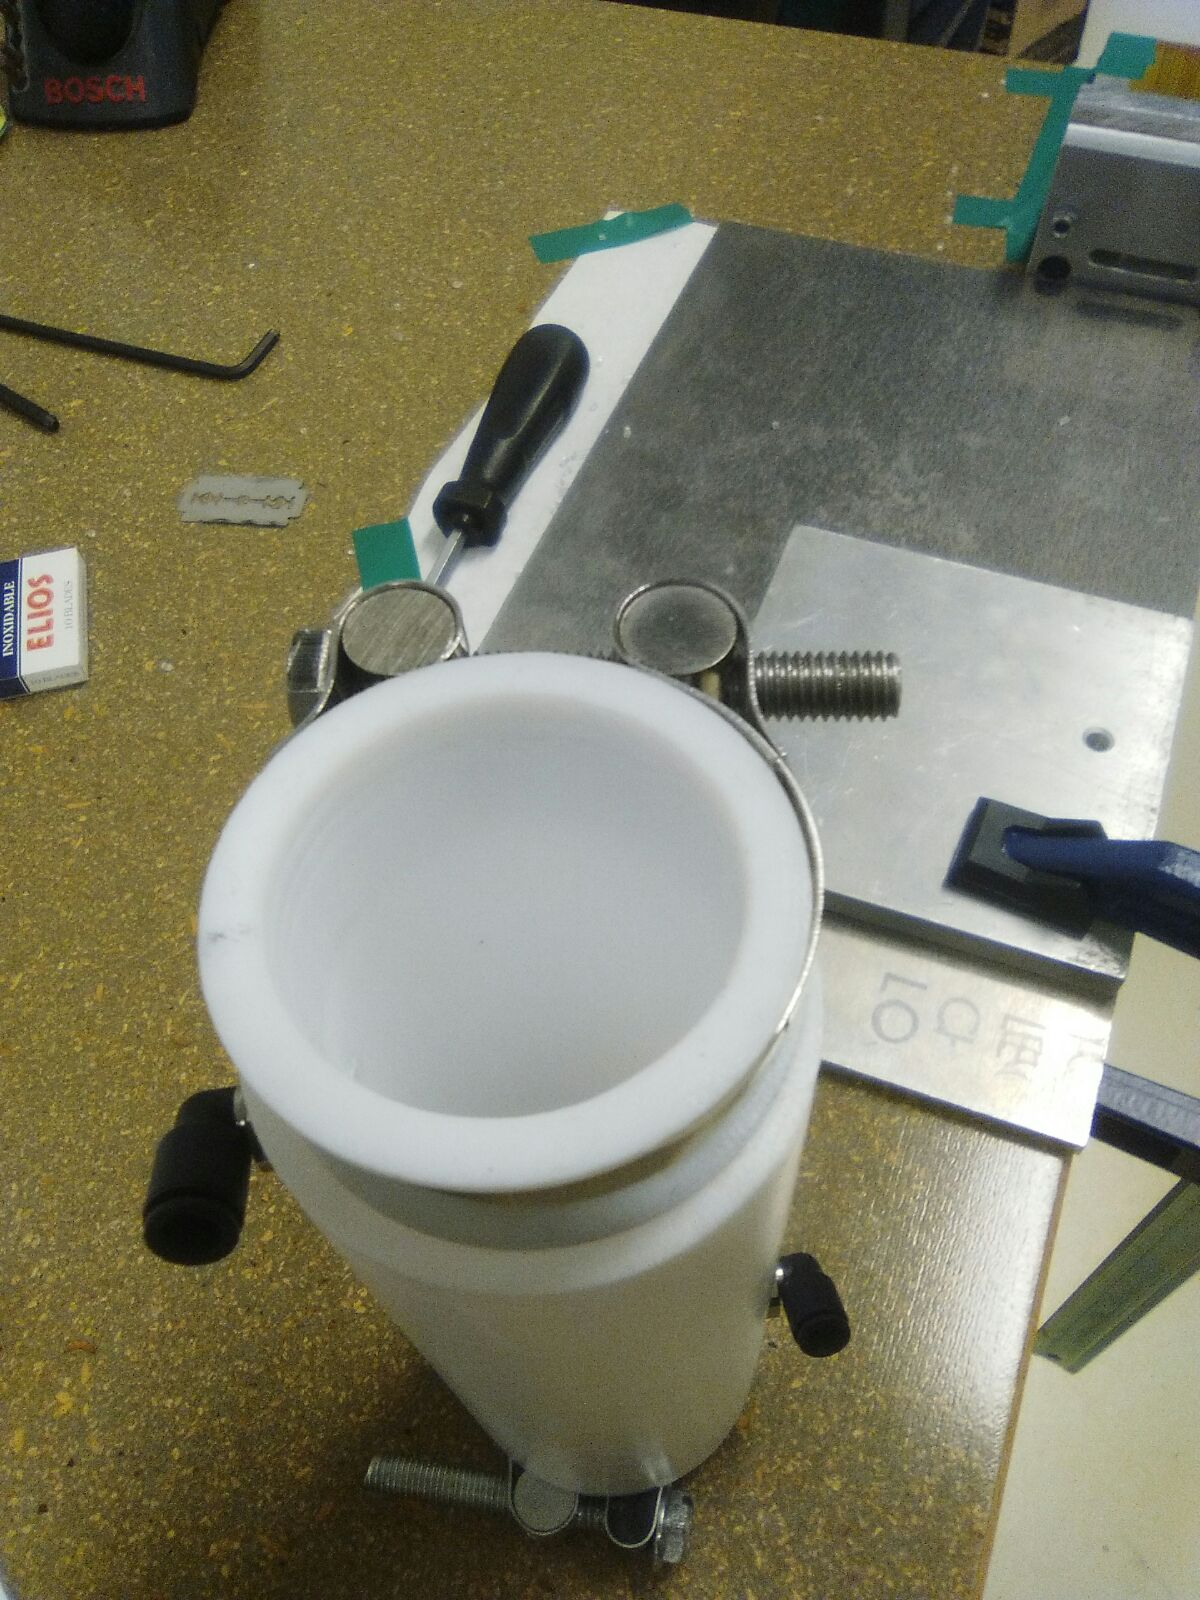
\includegraphics[width=0.5\textwidth]{AveiroPrototypeup.jpeg}}
 \caption{External cilinder of the Aveiro prototype. \label{externalcilinder}}
\end{figure}





\begin{figure}[hbtp]
\centering
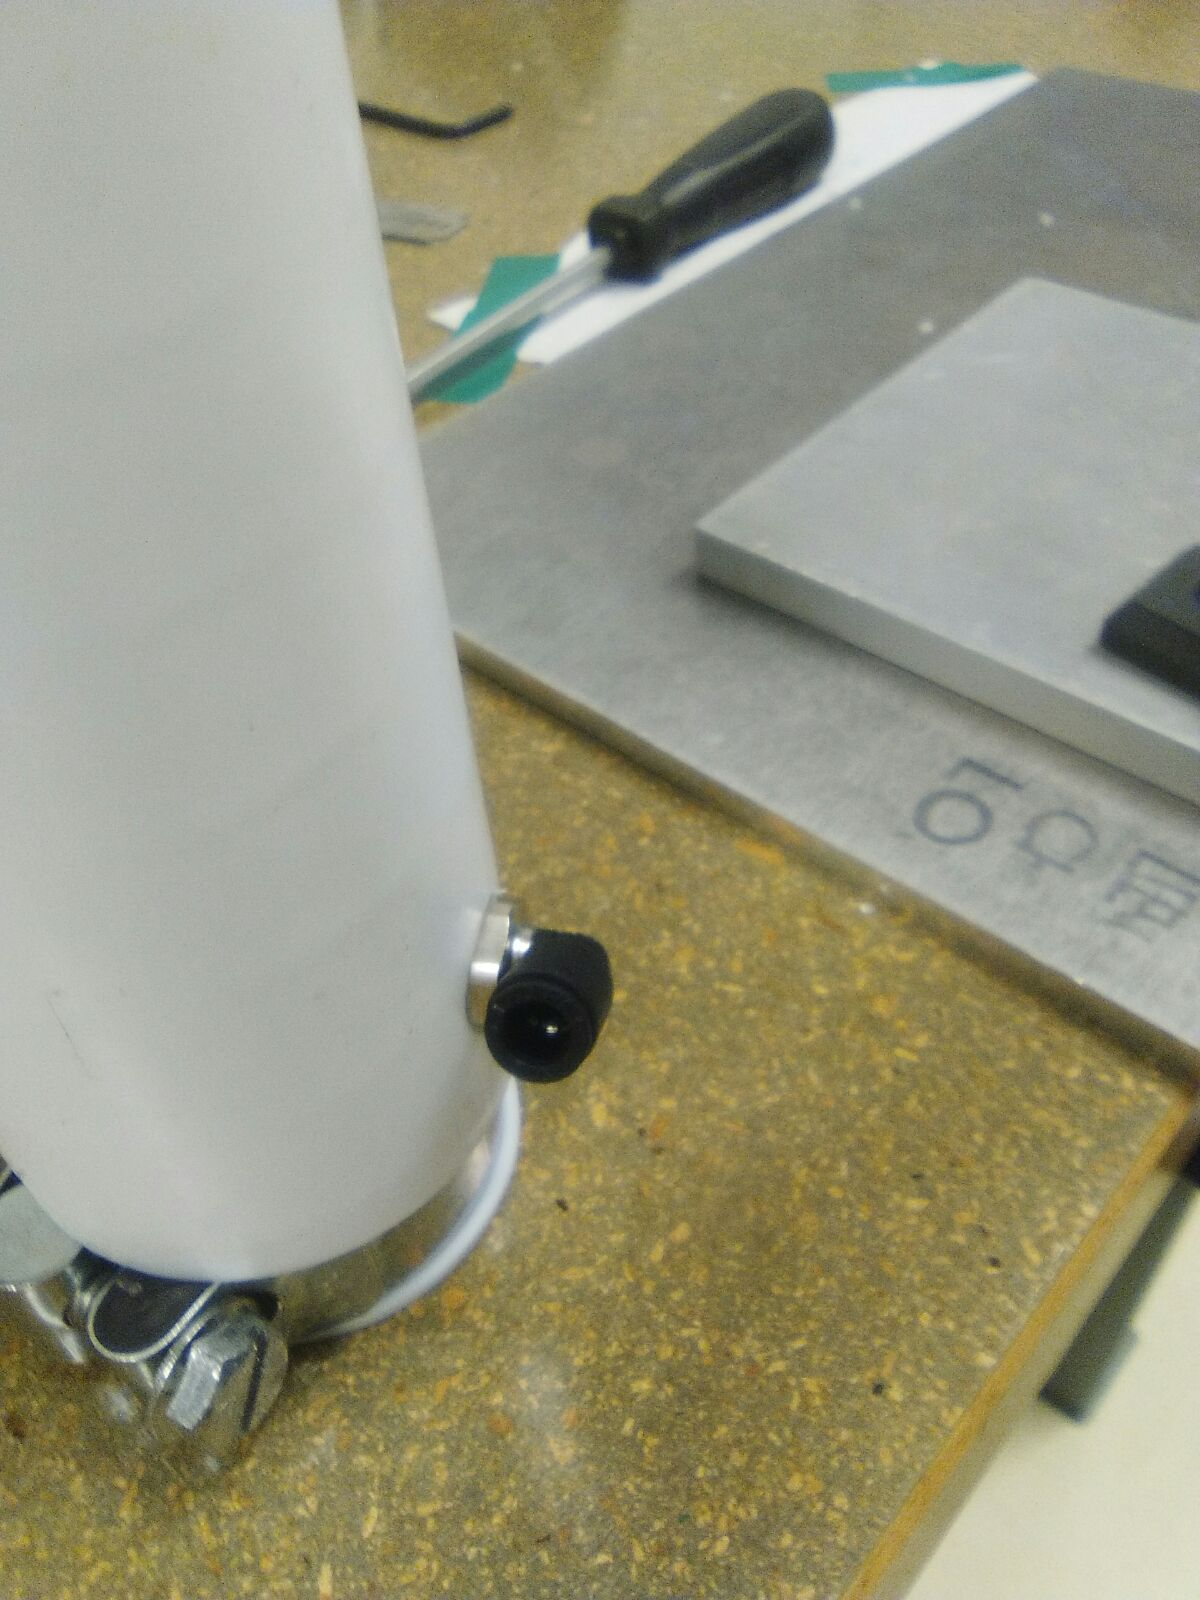
\includegraphics[scale=0.15]{hole.jpeg}
\caption{Filling and emptying holes \label{hole}}
\end{figure}

In the figure \ref{comparison} we can compare both, Aveiro (\ref{aveiro}) and Valencia (\ref{valencia}) prototype. There you can see that both prototypes have nearly the same external cilinder and their measurements are very close.  

\begin{figure}[hbtp]
 \centering
  \subfloat[Aveiro prototype\label{aveiro}]{
    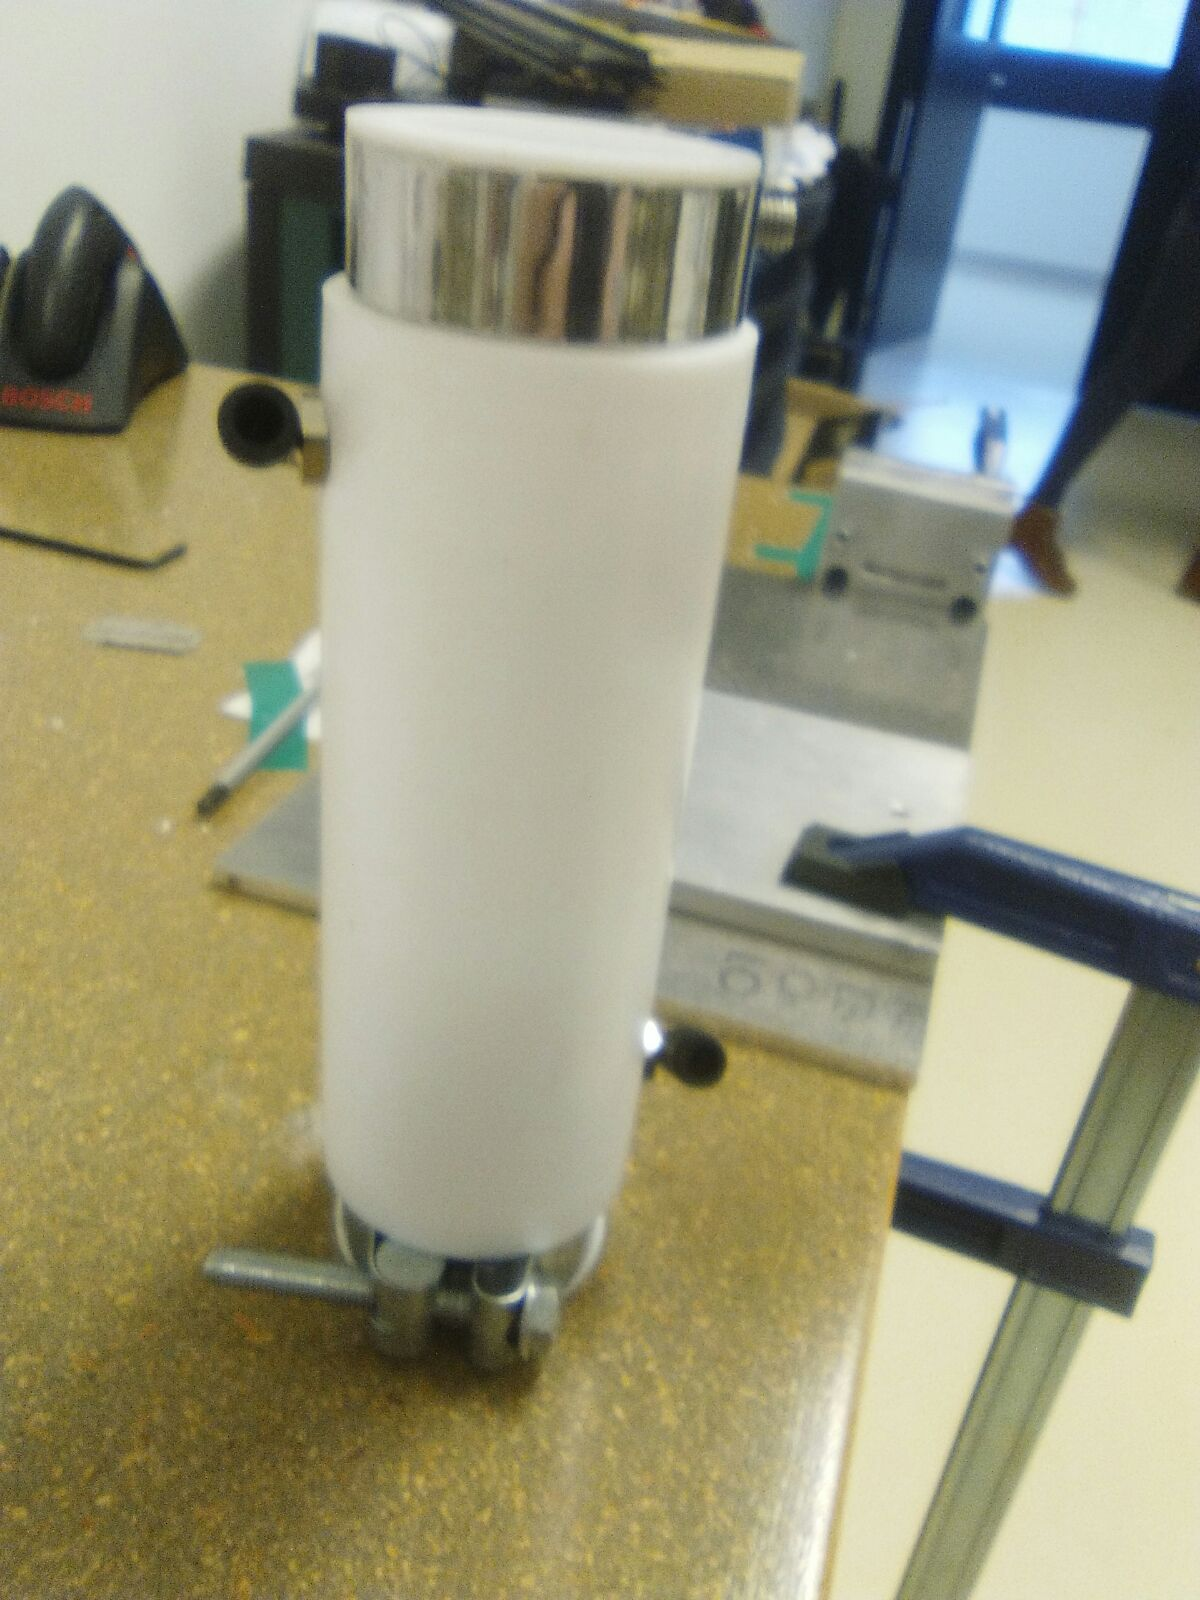
\includegraphics[width=0.5 \textwidth]{AveiroPrototype.jpeg}}
  \subfloat[Valencia prototype\label{valencia}]{
    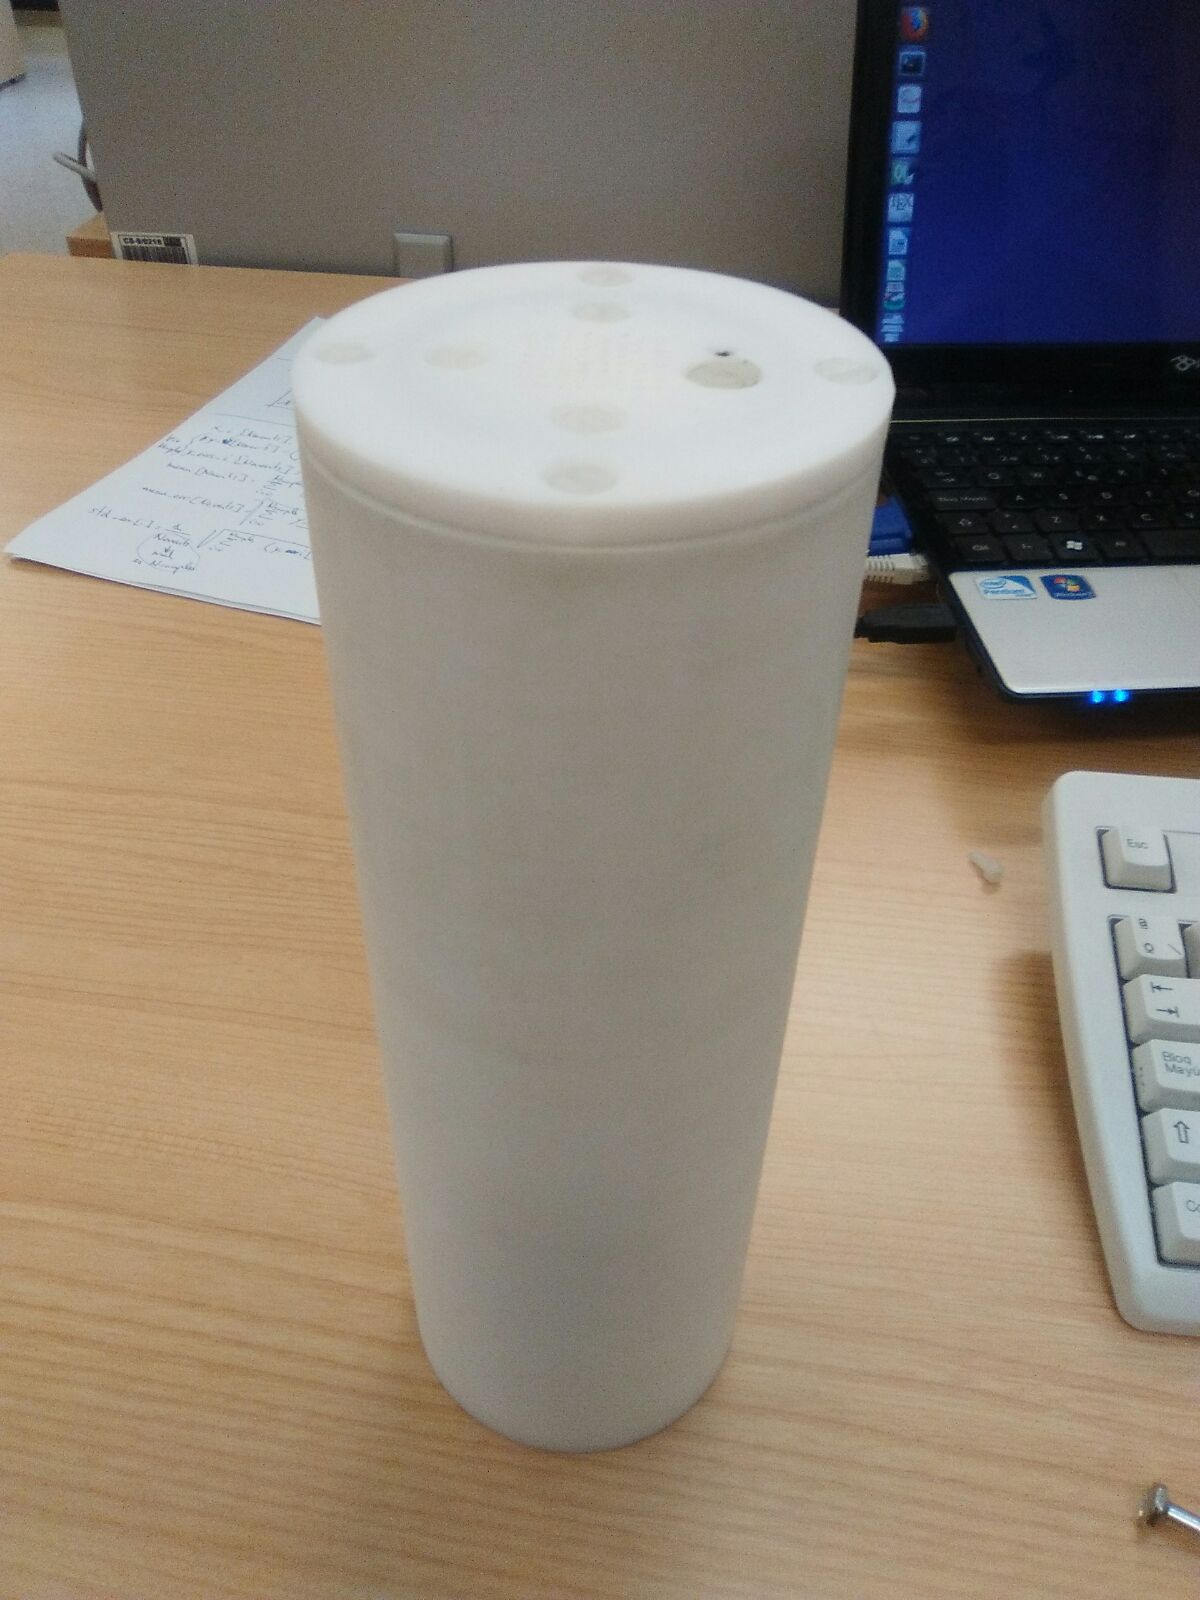
\includegraphics[width=0.5\textwidth]{ValenciaPrototype.jpg}}
 \caption{Comparison between prototypes \label{comparison}}
\end{figure}

The first difference between both prototypes is that the Valencia prototype uses fibers whose diameter is $1~\mm$ while the fibers, which are used by Aveiro prototype, is exactly the same type but with $2~\mm$ of diameter. It seems like a trivial difference but it is very important from point of view of physics. 

For doing a good election between both we have to take into account that we want to detect the electrons which are emitted by desintegration of tritium, whose mean free path is about $5$ or $6~\mu m$. Therefore, you could think that the best option is $1~\mm$ fibers because you can get a bigger active area (area which you can detect this electrons) since you can put more fibers in the same space. But the problem is that, if you use $1~\mm$ fibers you need to use a structure like the structure which appear in the figure \ref{structure}. 

\begin{figure}[hbtp]
\centering
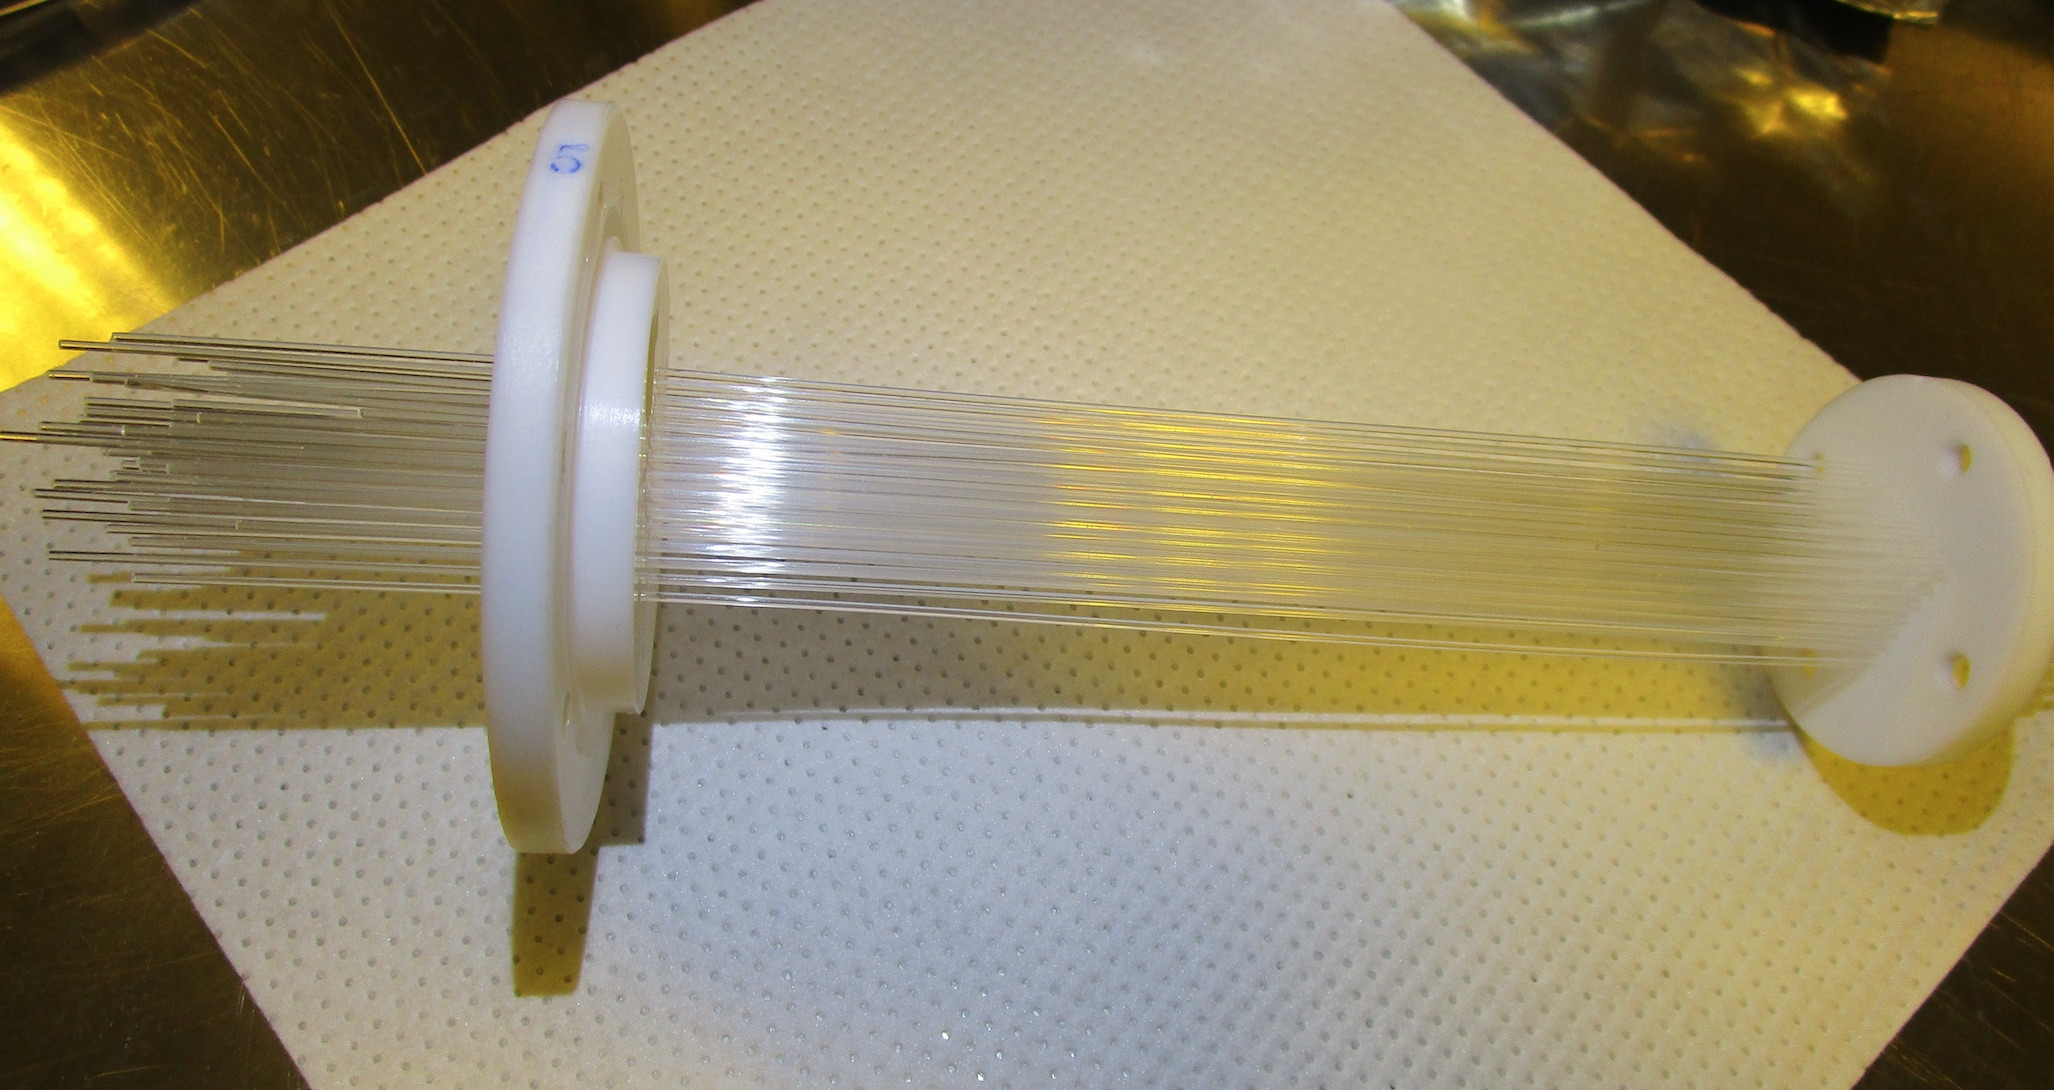
\includegraphics[scale=0.15]{structure.jpg}
\caption{Structure of the fibers of the valencia prototype \label{structure}}
\end{figure}


This structure is used by the Valencia prototype. The reason of this is that you need that your fibers are separated because if you don't do it, tritium water won't pass between your fibers so your active area will be less. You can avoid this problem if you use $2~\mm$ fibers because in this case, this size is enough for allowing that tiritum water pass between the fibers. In this case you have to take into account that fibers are touching each other and some of them are touching the teflon walls so your active area will be the total area of the fibers minus the area which is in contact between fibers.

In summary, if we use $1~\mm$ fibers we will have more active area in the same conditions but we need to use a structure for the fibers whereas if we use $2~\mm$ fibers, we will have less active area in the same conditions but we can avoid to use this structure so we can put more fibers in the same space for getting a bigger active area. Furthermore, $2~\mm$ fibers have more resistance which is very important because these will be subject to a continuous flow of water so we need that they are resistant.

In short, the Valencia prototype uses a structure that organize fibers whose diameter is $1~\mm$ while the aveiro prototype use $2~\mm$ fibers whitout any structure.

We can't estimate what is the best option because the contact area between fibers and between the fiber and the telfon walls will depend on the imperfection of the shape of every fiber since ideally it is a line, not a area and there's not exist any simulation program which can simulate these things. Moreover there are many other things which will affect in every configurate of the prototype differently like collection efficiency or signal-noise relation. You can't estimate it neither although you do several simulations of this experiment because it depends on the state of the surface of every fiber and the teflon walls. So the best option will be to put both prototypes in almaraz nuclear power plant and compare both results.

Next step will be to cut this $2~\mm$ fibers. It is more complex than $1~\mm$ fibers because if you use a thick blade you damage the fiber when you cut it but if you use a thin blade you damage the blade and it affect to your fiber. We tried to cut with several techniques and the only device, in which we were able to obtain a cutting optically acceptable, was with the cuttinc device which Valencia people developed and built in their workshop. In the figure \ref{cuttingdevice} you can observe this one.

\begin{figure}[hbtp]
 \centering
  \subfloat[]{
    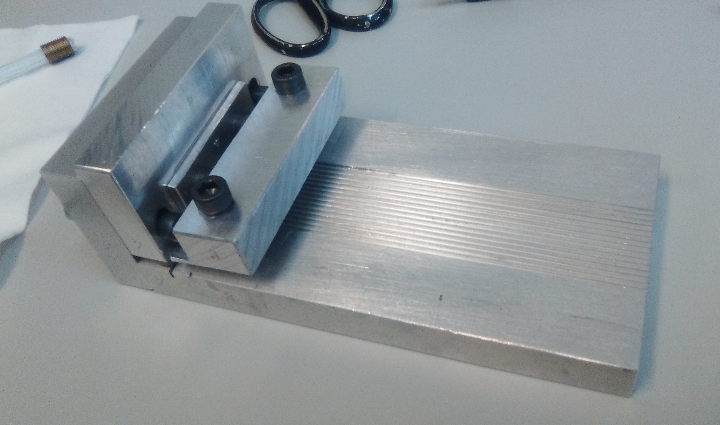
\includegraphics[width=0.5 \textwidth]{Guillotina1.png}}
  \subfloat[]{
    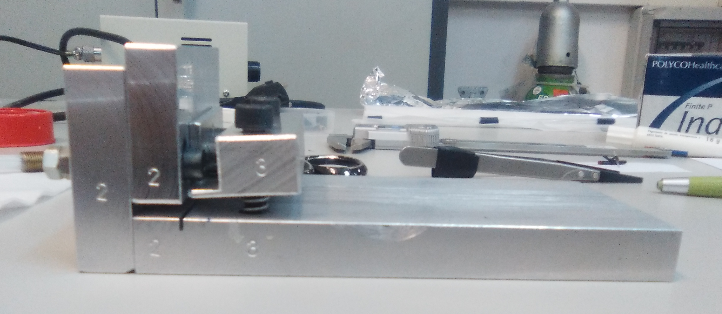
\includegraphics[width=0.5\textwidth]{Guillotina2.png}}
 \caption{Valencia cutting device \label{cuttingdevice}}
\end{figure}

We have to take into account that we need to do the transmission of the photons, which are creating inside the fibers due to tritium events, between this fibers, which will be inside the prototype in contact with tritium water, and the PMT or SiPM, which will be outside the prototype and it can't touch the tritium water. 

Doing this step in a correctly way is more easy for Valencia people than Aveiro people because the Valencia prototype uses a structure for hold every fiber so we can make several holes with the same matrix that this structure so that fibers through the prototype and it get out. Therefore, now, we only have to use optical grass to couple correctly this fibers to the photons counter. In the figure \ref{valenciaholes} you can see the cilinder cover which have this holes matrix.

\begin{figure}[hbtp]
 \centering
  \subfloat[Holes matrix of the valencia prototype]{
    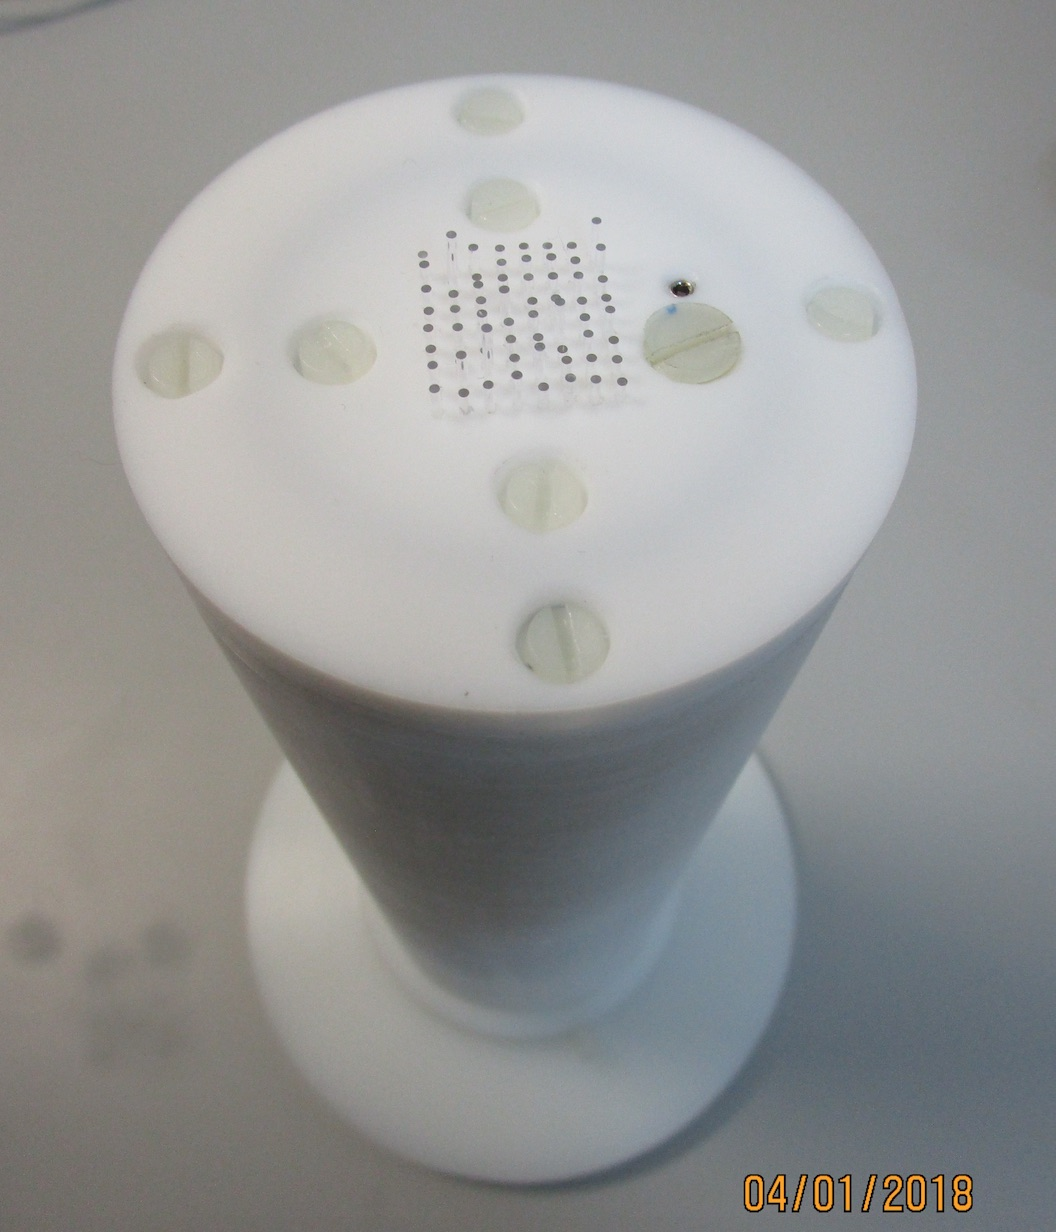
\includegraphics[width=0.5 \textwidth]{holesmatrix.jpg}}
  \subfloat[Holes matrix of the valencia prototype (zoom)]{
    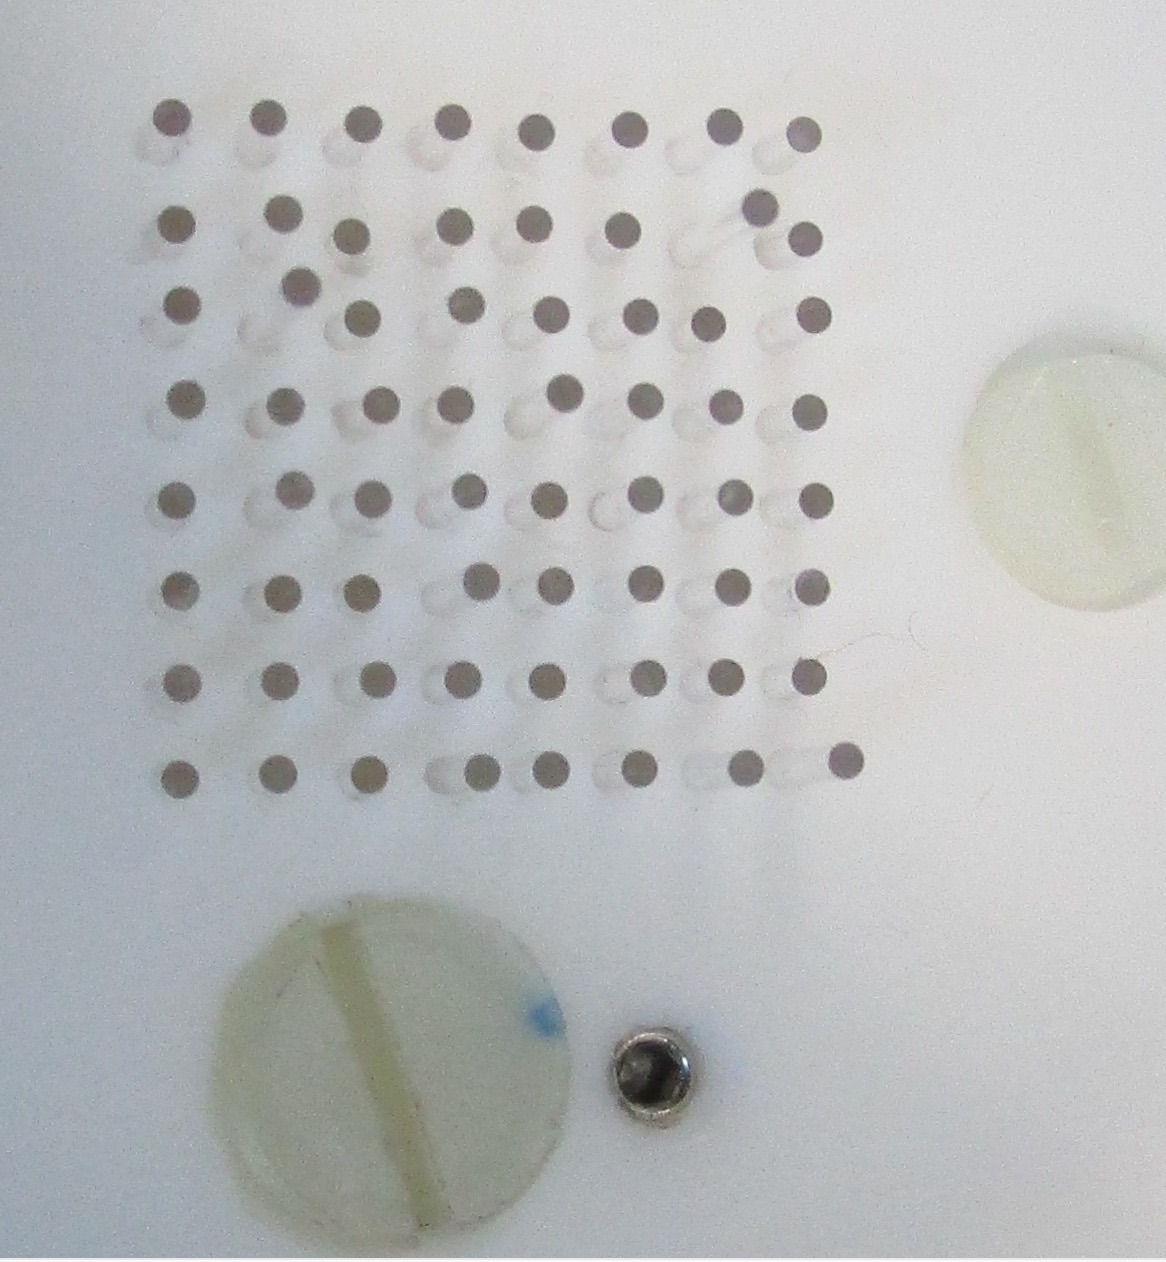
\includegraphics[width=0.5\textwidth]{holesmatrixzoom.jpg}}
 \caption{Holes matrix of the Valencia prototype \label{valenciaholes}}
\end{figure}

But Aveiro preople, contrary to Valencia people, can't do this because they don't have any structure of the fibers. Their idea for doing this task is to use a methacrylated glass (PMMA), which have a transmission coefficient clouse to 1 for this kind of photons, in every extrem of the prototype and it will be to fix with metalics belts which you can observe in the figure \ref{externalcilinder}. In this case you will can get that the photons through this glass whitout tritium water do it. Now, likewise valencia prototype, we only have to use optical grass to couple correctly this methacrylated glass to the photons counter. The length of this methacrylated glass is $10~\mm$ so the length of fibers, which will be inside, have to be $180~\mm$. We cut about $370$ fibers, of which about $350$ out of them we put inside the prototype. This is the number which we can put inside of this prototype without they being too narrow. You can see it in the figure \ref{fibers}. 

\begin{figure}[hbtp]
\centering
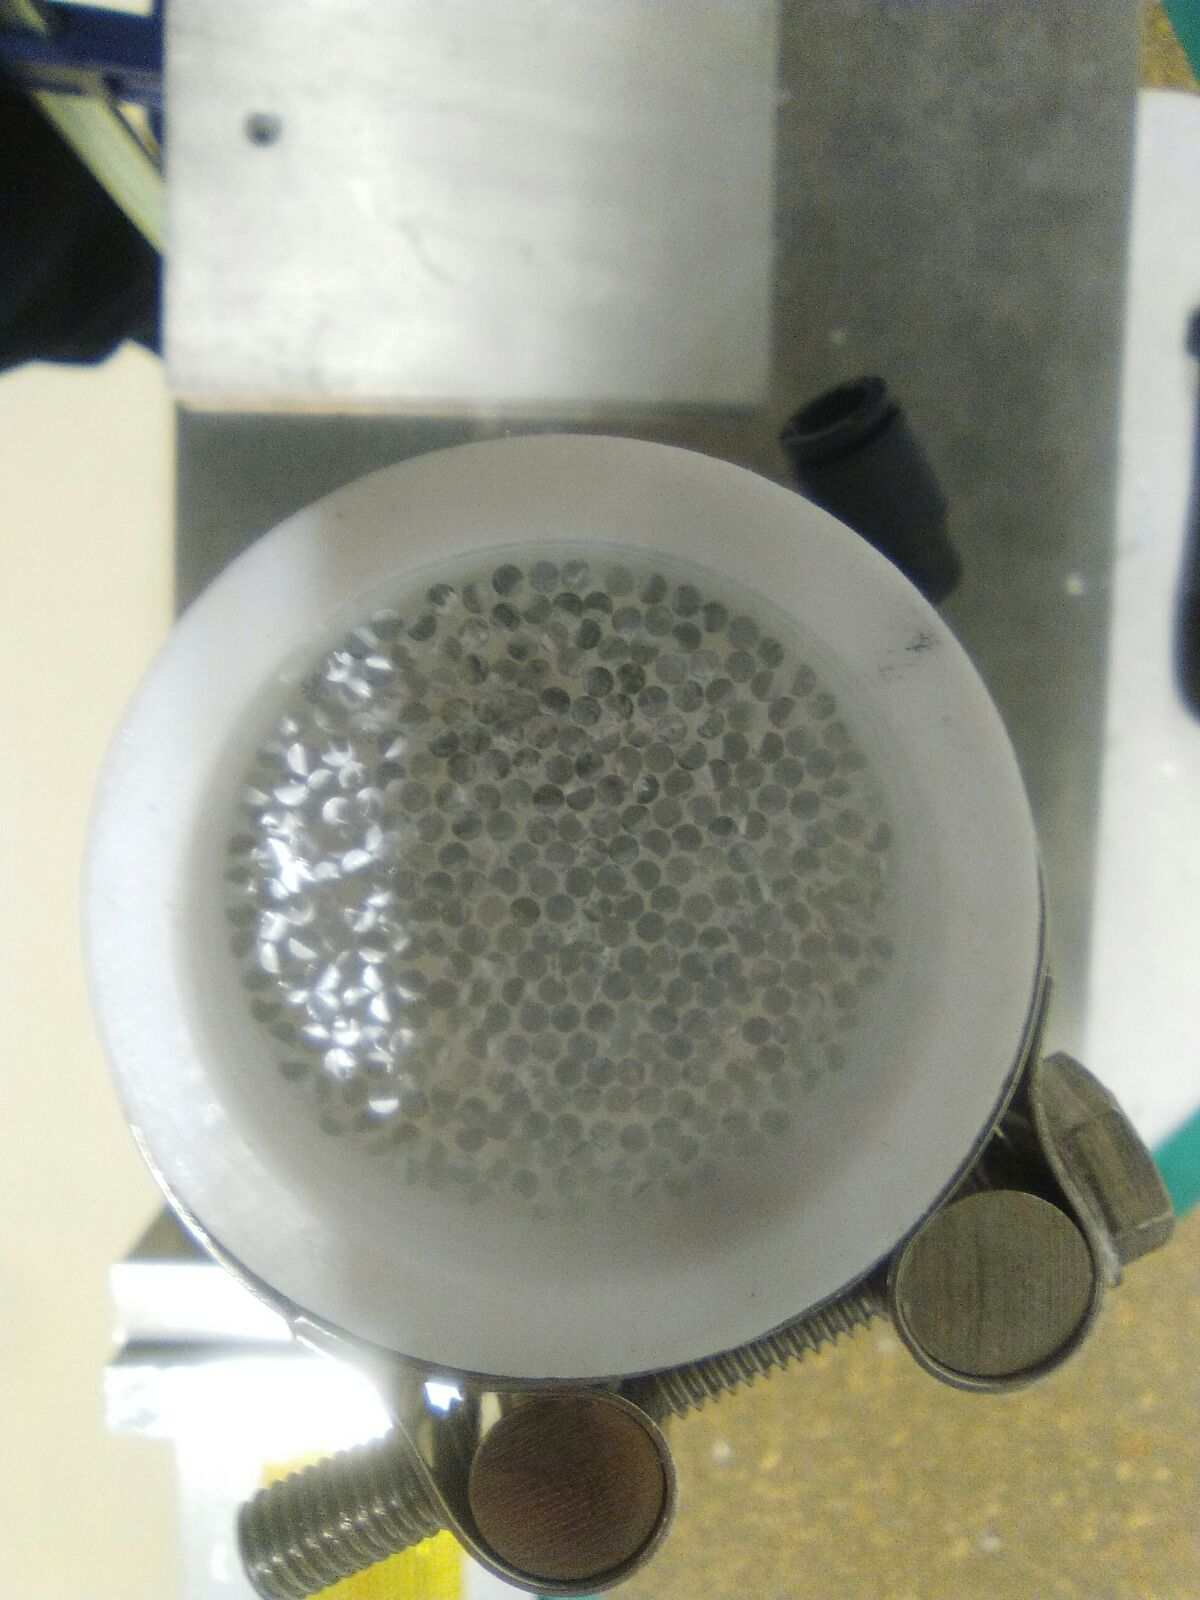
\includegraphics[scale=0.15]{fibers.jpeg}
\caption{Fibers inside the prototype \label{fibers}}
\end{figure}

We have seen that with this cutting device we have obtained a lower precision than $1~\mm$ in their length.

The Aveiro way for doing the transmission of the light have a problem which don't exit with the Valencia configuration. We can control quite good the conexion between fibers and photons counter for valencia prototype but, for aveiro prototype, we can control quite good the conexion between methacrylated glass and photons counter but we can't control the conexion between fibers and methacrylated glass because we can't use optical grass since it will be in contact with tritium water. It is a critical point because a bad conexion could produce a huge loss in our signal. 

Therefore we need that all fibers have exactly the same length for ensuring that all fibers will be in contact with both glass pieces correctly. As I said berfore, we can get a lower precision than $1~\mm$ in their length with our cutting devices but it isn't enough. Therefore we need to polish every fiber for two reasons.

\begin{itemize}
\item{} First we need to polish because in spite of we obtain a good final state with our cutting device we can improve this results if we polish fibers before that. It is very important because we can improve our signal which is essential in our experiemnt.
\item{} Second we need to polish because we can improve the presicion in the length of fibers. It is other essential thing in aveiro porotoype because we can improve the transmission of the light, which can affect to the signal a lot.
\end{itemize}

The thing is that until now we was polishing the fibers one by one handly and we had to spend 10 minuts more or less in every fiber. In the past we could do this because we work with few fibers but now we have $350$ fibers. You can see that we need too much time for doing this task so we though about some alternative way for doing this task efficiently. We look for in internet but there are not any comercial device which doing this so we have started to build a simply device which do this task and which have a precision better than $1~\mm$ in their length. In the section \ref{sec:polishing} of this report I will explain this device. 
